%%%%%%%%%% Page 2 - Col 1 %%%%%%%%%%
\newpage
\colorfulheader{\texttt{C++} programming}

\begin{minipage}[t]{0.485\textwidth}
    \colorfulsection{Arrays}
    \begin{itemize}[leftmargin=*]
        \setlength\itemsep{0pt}
        \item \inlinecode{type array\_name\bracket{\#elements}} $\mapsto$ declaration
        \item \inlinecode{array\_name\bracket{array\_index}} $\mapsto$ accessing
        \item Initialization does not need to be \quotes{complete}
        \begin{lstlisting}
            // For an array of length N the C indexing is as follow
            // Index    0   1   ...   N-1   N
            // Array [    |   | ... |     |   ]
            int foo[5] = {1, 2, 3, 4, 5} // [1, 2, 3, 4, 5]
            int foo[5] = {1, 2, 3} // [1, 2, 3, 0, 0]
            int foo[] = {1, 2, 3} // [1, 2, 3] Automatic size
            int foo[3] = {} // [0, 0, 0]
        \end{lstlisting}
        \item The \inlinecode{=} sign can be dropped for \textbf{universal initialization} \\
        \inlinecode{int foo[]\curlybracket{10, 20, 30}} $\mapsto$
        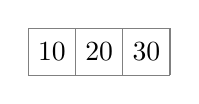
\begin{tikzpicture}[x=1cm, y=1cm, xscale=0.6, yscale=0.6, baseline=5.5pt]
        \draw[step=1cm, color=gray, thin] (0, 0) grid (3, 1);
        \node at (0.5, 0.5) {10};
        \node at (1.5, 0.5) {20};
        \node at (2.5, 0.5) {30};
        \end{tikzpicture}
        \item Can be \textbf{multidimensional} \inlinecode{data[\#rows][\#cols]}, for example \inlinecode{data[3][2]} is represented as
        \begin{customcenter}[0pt]
            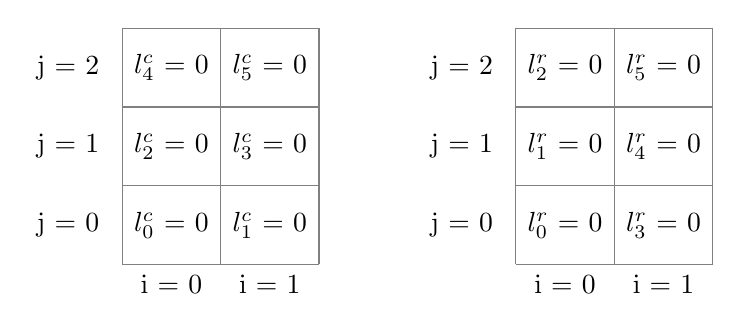
\begin{tikzpicture}[x=1cm, y=1cm, xscale=1.25, yscale=1]
                \draw[step=1cm, color=gray, thin] (0,0) grid (2, 3);
                \node at (-0.55, +0.50) {j = 0};
                \node at (-0.55, +1.50) {j = 1};
                \node at (-0.55, +2.50) {j = 2};
                \node at (+0.50, -0.25) {i = 0};
                \node at (+1.50, -0.25) {i = 1};
                \node at (0.5, 0.5) {$\text{l}_0^\text{c}$ = 0};
                \node at (1.5, 0.5) {$\text{l}_1^\text{c}$ = 0};
                \node at (0.5, 1.5) {$\text{l}_2^\text{c}$ = 0};
                \node at (1.5, 1.5) {$\text{l}_3^\text{c}$ = 0};
                \node at (0.5, 2.5) {$\text{l}_4^\text{c}$ = 0};
                \node at (1.5, 2.5) {$\text{l}_5^\text{c}$ = 0};
                \draw[step=1cm, color=gray, thin] (4, 0) grid (6, 3);
                \node at (3.45, +0.50) {j = 0};
                \node at (3.45, +1.50) {j = 1};
                \node at (3.45, +2.50) {j = 2};
                \node at (4.50, -0.25) {i = 0};
                \node at (5.50, -0.25) {i = 1};
                \node at (4.5, 0.5) {$\text{l}_0^\text{r}$ = 0};
                \node at (4.5, 1.5) {$\text{l}_1^\text{r}$ = 0};
                \node at (4.5, 2.5) {$\text{l}_2^\text{r}$ = 0};
                \node at (5.5, 0.5) {$\text{l}_3^\text{r}$ = 0};
                \node at (5.5, 1.5) {$\text{l}_4^\text{r}$ = 0};
                \node at (5.5, 2.5) {$\text{l}_5^\text{r}$ = 0};
            \end{tikzpicture}
        \end{customcenter}
        \begin{lstlisting}
            // Elements of array data[3, 2] can be
            // accessed/computed as
            for (int i = 0; i < 2; i++)
            for (int j = 0; j < 3; j++)
            int linear_index_c = (i + j * 2); // Slow accessing?
            int linear_index_r = (j + i * 3); // Fast accessing?
            data[j][i] = 0; // Accessing with 2 indices
            data[linear_index_c] = 0; // Accessing linearly - col
            data[linear_index_r] = 0; // Accessing linearly - row
        \end{lstlisting}
        \item As function parameters
        \begin{lstlisting}
            // one-dimensional, size can be left blank 
            void procedure(int arg[]) {}
            // multi-dimensional, 2nd or more dimensions requires 
            // size aka memory layout
            void procedure(int array[][3]) {}
        \end{lstlisting}
        \item An alternative for raw arrays in \inlinecode{C++} is the container \inlinecode{std::array<type, size>}, which can be accessed via the \inlinecode{\#include <array>} header
    \end{itemize}
    \colorfulsection{Pointers}
    \begin{itemize}[leftmargin=*]
        \item \inlinecode{type *} represents a \textbf{pointer} to a type
        \item \inlinecode{\&} is the \textbf{reference} operator and can be read as \quotes{address of}
        \item \inlinecode{*} is the \textbf{dereference} operator and can be read as \quotes{value pointed by}
        \begin{lstlisting}
        int var = 25; // Initial variable var with value 25
        int * foo = &var; // foo points to the address of var
        int bar = var; // bar is a new variable of value var
        int baz = *foo; // baz dereference foo, gets 25
        \end{lstlisting}
    \end{itemize}
\end{minipage}
%%%%%%%%%%%%%%%%%%%%%%%%%%%%%%%%%%%%
\hspace{10pt}
%%%%%%%%%% Page 2 - Col 2 %%%%%%%%%%
\begin{minipage}[t]{0.485\textwidth}
    \begin{itemize}[leftmargin=*]
        \setlength\itemsep{0pt}
        \item Pointers can be manipulated \quotes{arithmetically}
        \begin{lstlisting}
            void console_log_p(int * p) { printf("%p:%d, ", p, *p); }
            int main() 
            {
                int numbers[5];
                int * p;
                p = numbers; *p = 10; console_log_p(p);
                p++; *p = 20; console_log_p(p);
                p = &numbers[2]; *p = 30; console_log_p(p);
                p = (numbers + 3); *p = 40; console_log_p(p);
                p = numbers; *(p + 4) = 50; console_log_p(p);
                return; 
            }
        \end{lstlisting}
        Suppose \inlinecode{0x567} is the address of \inlinecode{p}, above code prints
        \emptyline
        \inlinecode{0x567:10, 0x56A:20, 0x56E:30, 0x572:40, 0x576:50}
        \item \quotes{Constantsy} of pointers
        \begin{lstlisting}
            int x; // non-const int variable
            int* p1 = &x; // non-const pointer to non-const int
            const int* p2 = &x; // non-const pointer to const int
            int* const p3 = &x; // const pointer to non-const int
            const int* const p4 = &x; // const pointer to const int
        \end{lstlisting}
        \item String literals (\quotes{text}) can be represented as \\ \inlinecode{const char * foo = \quotescode{hello}}
        \begin{customcenter}[0pt]
            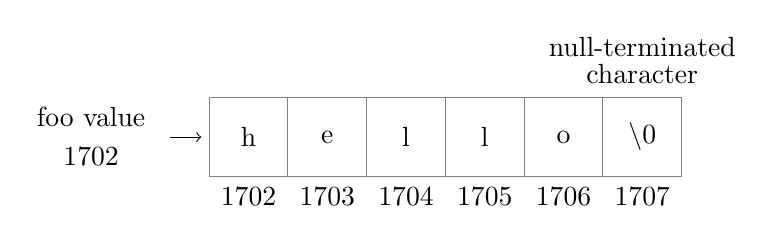
\begin{tikzpicture}
                \node at (-1.5, 0.75) {foo value};
                \node at (-1.5, 0.25) {1702};
                \draw[->] (-0.5, 0.5) -- (-0.1, 0.5);
                \draw[step=1cm, color=gray, thin] (0,0) grid (6, 1);
                \node at (0.5, 0.5) {\charactercode{h}};
                \node at (1.5, 0.5) {\charactercode{e}};
                \node at (2.5, 0.5) {\charactercode{l}};
                \node at (3.5, 0.5) {\charactercode{l}};
                \node at (4.5, 0.5) {\charactercode{o}};
                \node at (5.5, 0.5) {\charactercode{\textbackslash0}};
                \node at (0.5, -0.25) {1702};
                \node at (1.5, -0.25) {1703};
                \node at (2.5, -0.25) {1704};
                \node at (3.5, -0.25) {1705};
                \node at (4.5, -0.25) {1706};
                \node at (5.5, -0.25) {1707};
                \node at (5.5, +1.65) {null-terminated};
                \node at (5.5, +1.30) {character};
            \end{tikzpicture}
        \end{customcenter}
        \item A pointer can point to a pointer
        \begin{lstlisting}
            char a; a = 'z'; // a has value of character z
            char * b; b = &a; // b points to a
            char ** c; c = &b; // c points to b
        \end{lstlisting}
        \item Initialization \inlinecode{int * p = 0; int * q = nullptr;} \\
        \inlinecode{nullptr} $\mapsto$ points to \quotes{nowhere} \\
        \inlinecode{void *} $\mapsto$ can point to somewhere
        \item Pointer to function \\ \inlinecode{type \parenthesis{*name}(parameters) = function\_name;}
    \end{itemize}
    \colorfulsection{Dynamic Memory}
    \begin{itemize}[leftmargin=*]
        \setlength\itemsep{0pt}
        \item Uses keyword \inlinecode{new} to allocate memory as in \\ \inlinecode{pointer = new type} or \inlinecode{pointer = new type\bracket{\#elements}}
        \item To release memory use \inlinecode{delete} or \inlinecode{delete[]} keyword
        \begin{lstlisting}
            int * poo = new int; // Allocate an int
            *poo = 1;  // Populate with 1
            int * foo = new int[5] // An array of 5 elements
            int elements = 3;
            int * hoo = new int[elements] // An array of 3 elements
            // Clear memory in reverse order
            delete[] hoo;
            delete[] foo;
            delete poo;
        \end{lstlisting}
        \item \inlinecode{C} can handle dynamic memory using \inlinecode{malloc}, \inlinecode{calloc}, \inlinecode{realloc} functions but requires the \inlinecode{\#include<cstdlib>} header
    \end{itemize}
\end{minipage}
%%%%%%%%%%%%%%%%%%%%%%%%%%%%%%%%%%%%